\section{Why the characters fail}
\label{sec:why}

The characters share three properties at once: they are dense, they share structure beyond density, and 18 patterns is a substantial load for 144 neurons. Fig.~\ref{fig:chars} places random subsets of the characters (200 per size, sizes 2 to 18, fresh 10\% noise) on the synthetic curves. The study does not vary the three properties factorially, so it cannot say how much of the failure each causes. It can say what each does alone.

\emph{Density is enough to break plain Hebbian.} Independent bits at density 0.80 give Hebbian $P_{50}$ \N{c:biased:0.8:hebb:10}, with recall \N{r:biased:0.8:hebb:10:18} at 18 patterns under either update. At the characters' density, independent bits would have an overlap of \N{d:overlap_indep}, most of the characters' \N{d:overlap_mean}.

\emph{Fixing density does not fix the characters.} The covariance rule removes the density effect on independent bits, yet on character subsets its $P_{50}$ is only \N{sp:cov:10} [\N{sp:cov:10:lo}, \N{sp:cov:10:hi}], and its recall at 18 is \N{s:18:cov:10}. That $P_{50}$ lies between the rule's values on prototype sets at $\rho = 0.2$ (\N{c:proto:0.2:cov:10}) and $\rho = 0.3$ (\N{c:proto:0.3:cov:10}). It is consistent with the characters' Pearson correlation of \N{d:pearson_mean} and with \N{d:all_on} pixels being on in all 18. The characters' densities also vary, from \N{d:dens_min}\% to \N{d:dens_max}\%, which the rule's single mean does not remove, and the study did not separate that from shared structure. So the characters carry shared structure beyond their density, and that structure and their uneven densities likely break the covariance rule together.

\emph{Plain Hebbian behaves as the characters' total overlap predicts.} On character subsets, recall at three patterns is \N{s:3:hebb:10} [\N{s:3:hebb:10:lo}, \N{s:3:hebb:10:hi}], between prototype sets at $\rho = 0.4$ (\N{r:proto:0.4:hebb:10:3}) and $\rho = 0.5$ (\N{r:proto:0.5:hebb:10:3}) and below independent bits at density 0.80 (\N{r:biased:0.8:hebb:10:3}). Storkey's subset $P_{50}$, \N{sp:storkey:10} [\N{sp:storkey:10:lo}, \N{sp:storkey:10:hi}], is close to its value at $\rho = 0.5$, \N{c:proto:0.5:storkey:10} [\N{c:proto:0.5:storkey:10:lo}, \N{c:proto:0.5:storkey:10:hi}].

\emph{Load matters, too, and the most for the assignment's update.} With the 0/1 update, 18 patterns are past the 50\% load even for random balanced patterns ($P_{50}$ \N{c:proto:0.0:hebb01:10}, recall \N{r:proto:0.0:hebb01:10:18} at 10\% noise and \N{r:proto:0.0:hebb01:20:18} at 20\%), so load alone would break the baseline as run. With the standard update, 18 is below the measured $P_{50}$ of \N{c:proto:0.0:hebb:10}, and load alone costs about a quarter of the patterns at 10\% noise (recall \N{r:proto:0.0:hebb:10:18}) and over a third at 20\% (\N{r:proto:0.0:hebb:20:18}).

\begin{figure}[t]
\centering
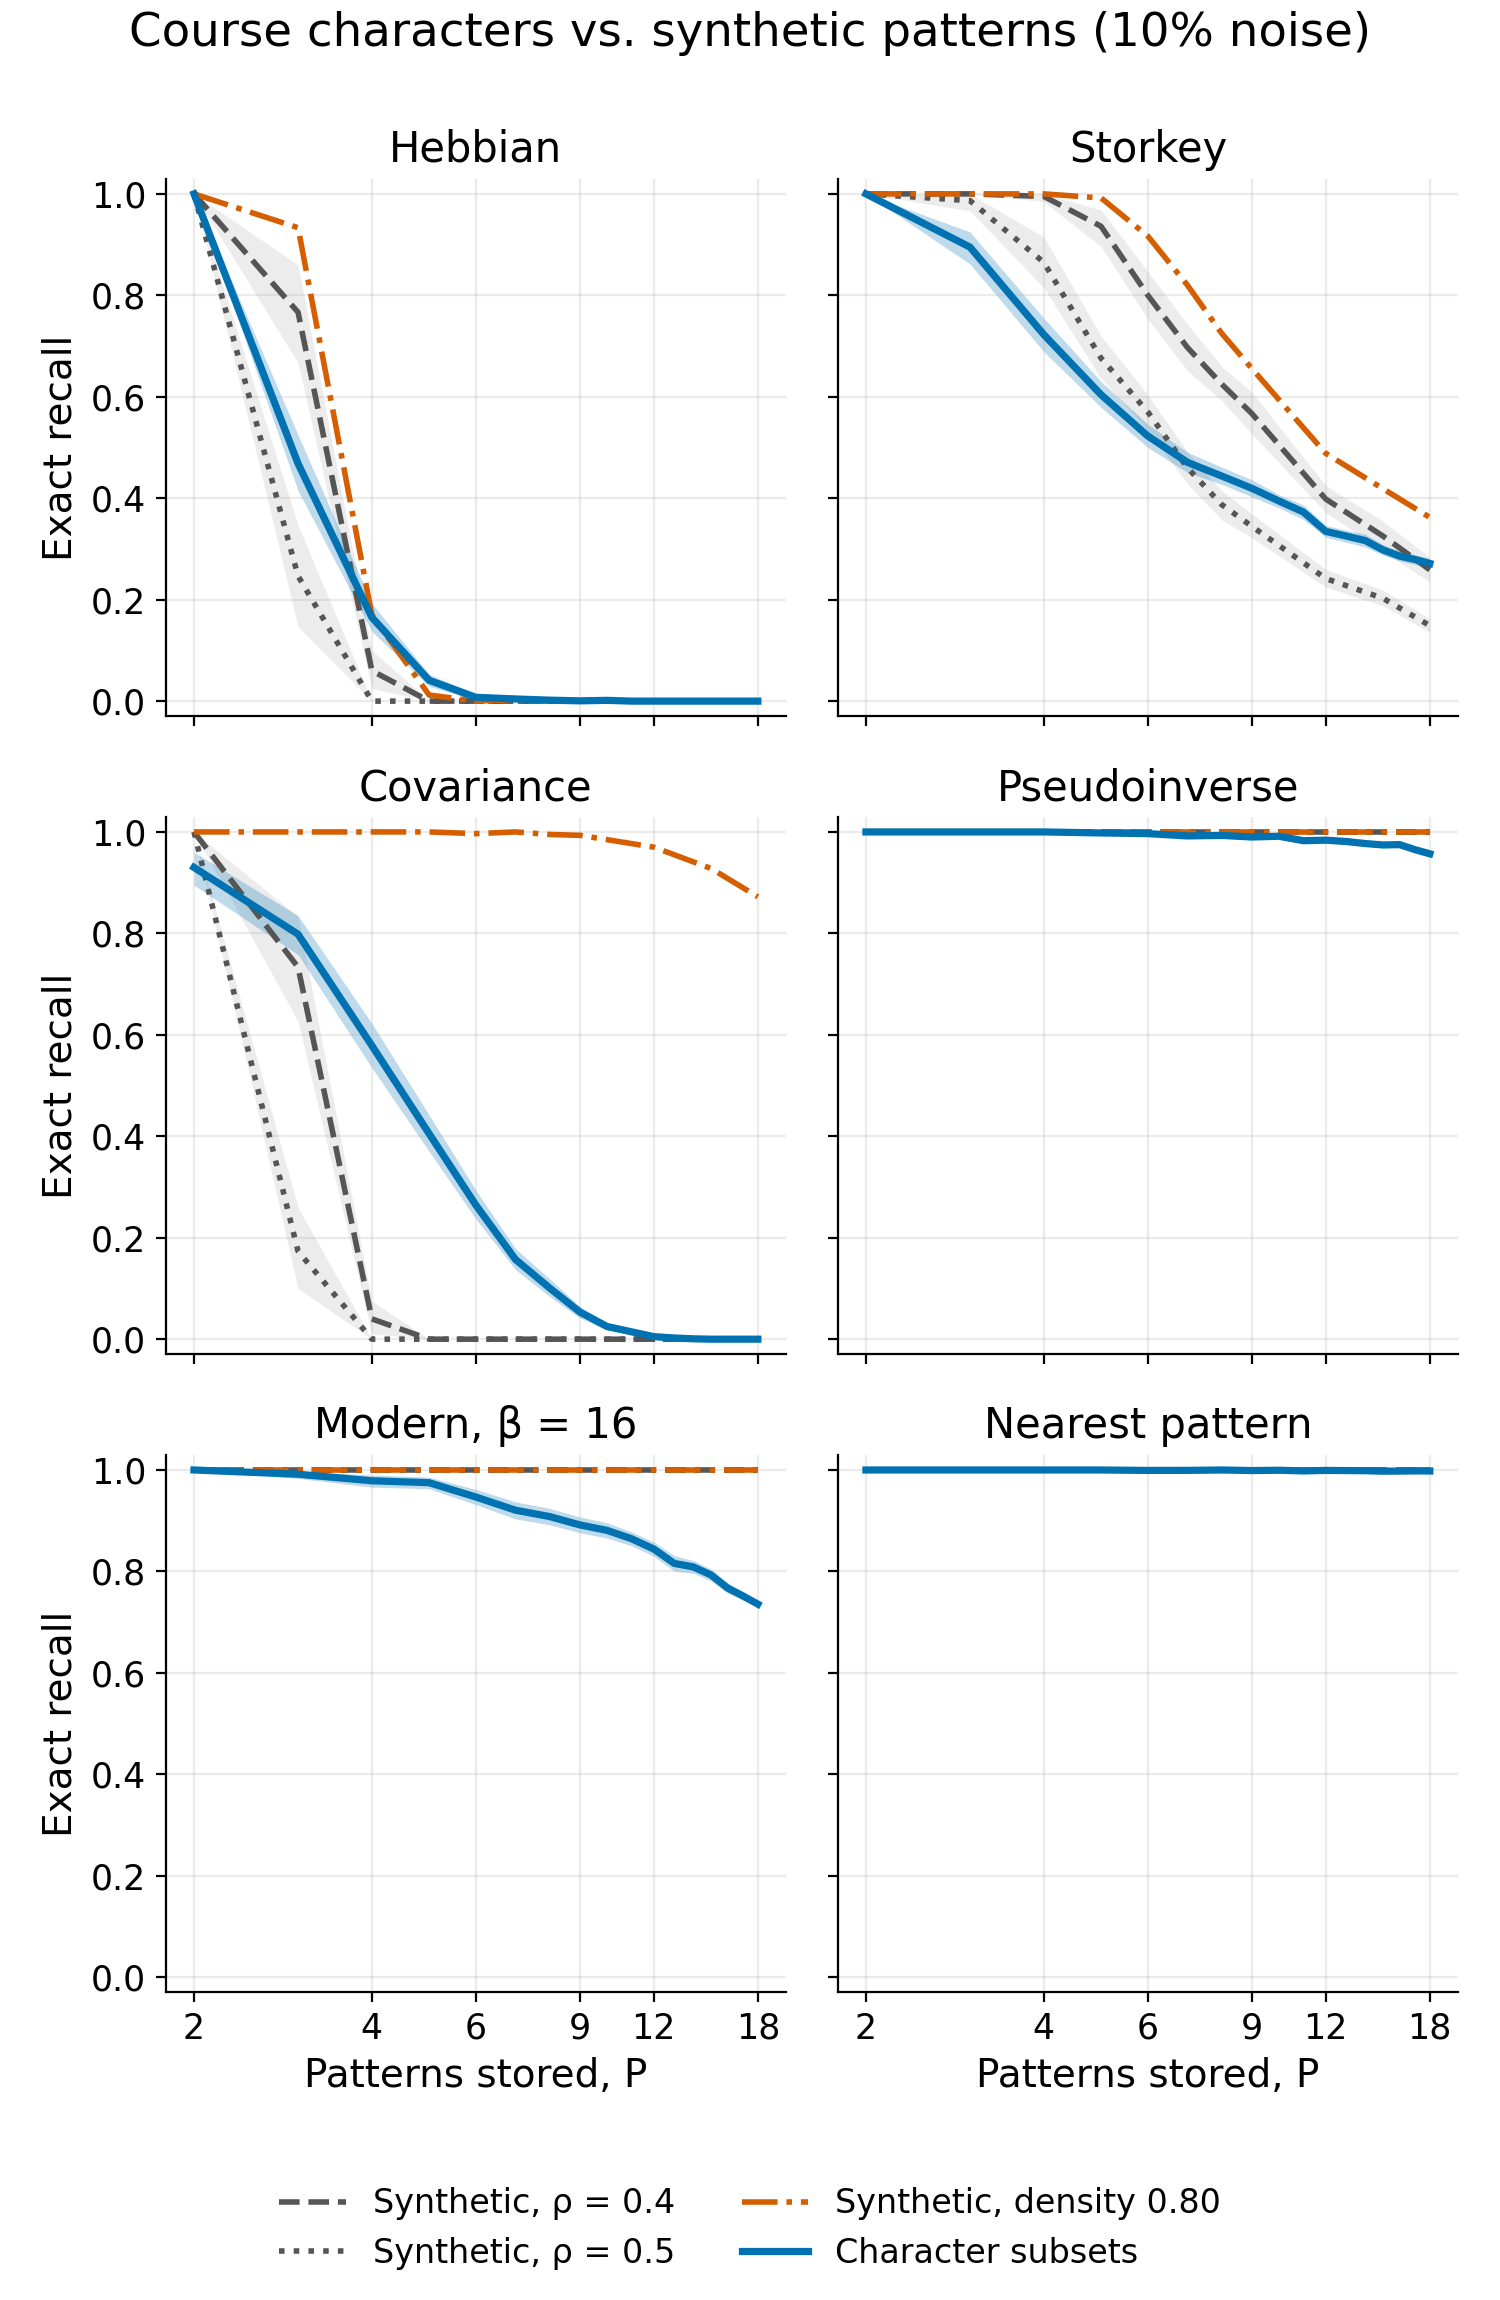
\includegraphics[width=\columnwidth]{../study/figures/fig4_characters_vs_synthetic.png}
\caption{Exact recall of random character subsets (solid) against synthetic patterns at $\rho = 0.4$ and $0.5$ and at density 0.80, 10\% noise.}
\label{fig:chars}
\end{figure}

\emph{For the strong rules, the characters are harder than their mean overlap suggests.} On the full set of 18, in the subset runs (a separate 200 draws from Table~\ref{tab:characters}'s), the pseudoinverse rule recalls \N{s:18:pinv:10} of the characters at 10\% noise and \N{s:18:pinv:20} at 20\%, while synthetic patterns at $\rho = 0.4$ and $0.5$ give \N{r:proto:0.4:pinv:10:18} and \N{r:proto:0.5:pinv:10:18} at 10\% and \N{r:proto:0.4:pinv:20:18} and \N{r:proto:0.5:pinv:20:18} at 20\%. The modern network at $\beta = 16$ recalls \N{s:18:modern16:10} of the characters at 10\% against \N{r:proto:0.4:modern16:10:18} on both synthetic levels. A likely cause is the characters' close pairs, with overlaps up to \N{d:overlap_max} and two patterns only \N{d:ham_min} bits apart, which a mean overlap does not capture. This is an interpretation. The study did not vary the distribution of overlaps separately.
